\section{Binäre Suche}


\begin{frame}[fragile]
\frametitle{Binäre Suche - Ziel}
\begin{itemize}
    \item Ziel: Finde die Position eines bestimmten Elements in einem sortierten Array.
\end{itemize}
\end{frame}

\begin{frame}[fragile]
\frametitle{Beispiel: Suche nach der Zahl 8 }
\begin{center}
     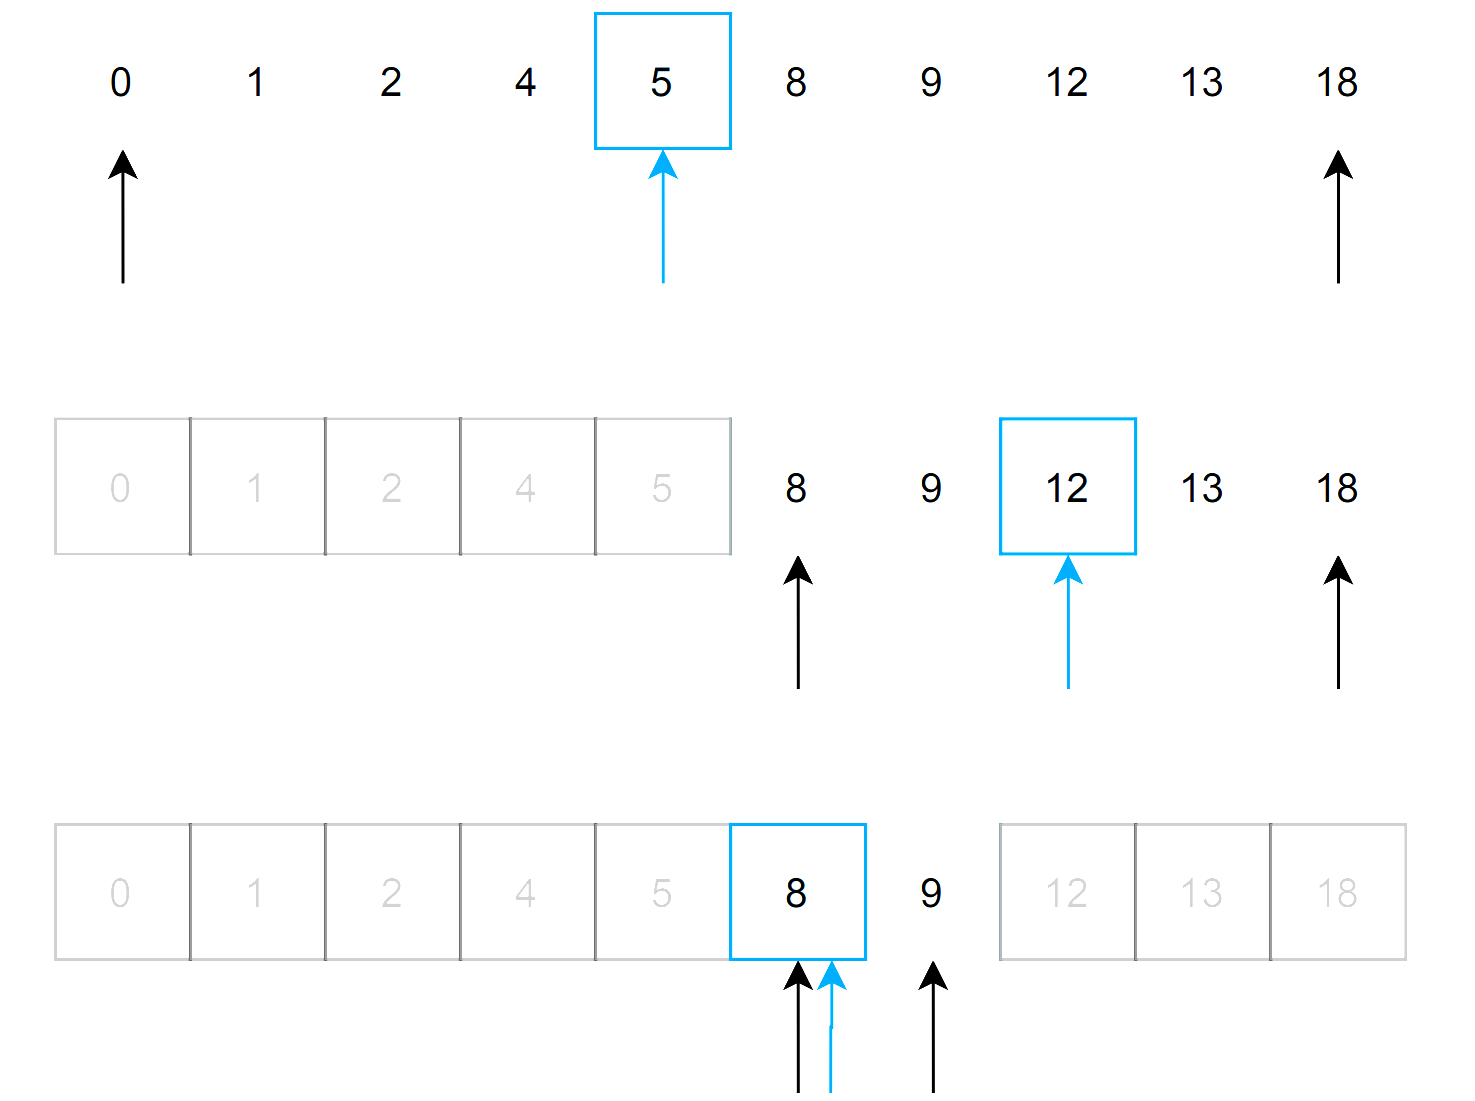
\includegraphics[height=0.7\textheight]{images/binSearchHappyCase}
\end{center}
\end{frame}

\begin{frame}[fragile]
\frametitle{Beispiel: erfolglose Suche nach der Zahl 8 }
\begin{center}
     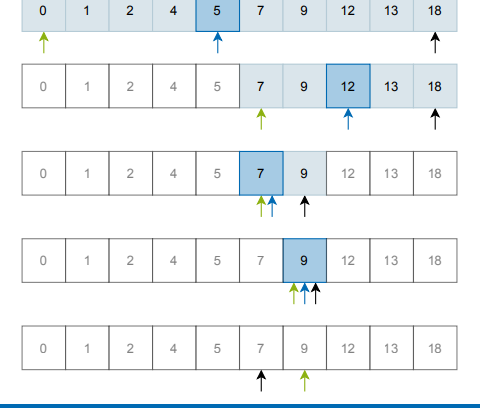
\includegraphics[height=0.7\textheight]{images/binSearchBadCase}
\end{center}
\end{frame}

\begin{frame}[fragile]
\frametitle{Binäre Suche - Beispiel}
\begin{lstlisting}
    int[] myArray = {1,4,5,6,8,8,10};
    int gesuchteZahl = 5;
\end{lstlisting}
\begin{enumerate}
    \item Mittleres Element: 6 (Index 3)
    \item 5 < 6, also suchen wir im linken Teil: \{1, 4, 5\}
    \item Mittleres Element: 4 (Index 1)
    \item 5 > 4, also suchen wir im rechten Teil: \{5\}
    \item Mittleres Element: 5 (Index 2)
    \item Zahl gefunden! Index: 2
\end{enumerate}
\end{frame}

\begin{frame}[fragile]
\frametitle{Binäre Suche Aufgaben}
\begin{itemize}
    \item wie viele Iterationen benötigen wir im schlechtesten möglichen Fall?
    \item Implementieren Sie Binäre Suche
    \item für schnelle: können sie das auch Rekursiv implementieren?
\end{itemize}  
\end{frame}